
\documentclass[11pt]{article}

% --------------------------------------------------------------------------
% Packages
% --------------------------------------------------------------------------
\usepackage[T1]{fontenc}
\usepackage[utf8]{inputenc}
\usepackage[margin=1in]{geometry}
\usepackage{ifthen}
\usepackage{microtype}
\IfFileExists{newtxtext.sty}{\usepackage{newtxtext,newtxmath}}{\usepackage{lmodern}}
\usepackage{setspace}
\usepackage{xspace}
\usepackage{parskip}
\usepackage{amsmath,mathtools}
\usepackage{booktabs,longtable,array,tabularx,multirow}
\usepackage{enumitem}
\usepackage[svgnames,table]{xcolor}
\usepackage{graphicx}
\usepackage{tikz}
\usetikzlibrary{arrows.meta,positioning,fit,shapes.geometric,calc,backgrounds,patterns,decorations.pathreplacing}
\usepackage[most]{tcolorbox}
\usepackage{titlesec}
\usepackage{fancyhdr}
\usepackage{float}
\usepackage{listings}
\usepackage{caption}
\usepackage{subcaption}
\usepackage[hidelinks]{hyperref}
\usepackage[backend=biber,style=numeric-comp,sorting=none,maxbibnames=6]{biblatex}
\addbibresource{bib/references.bib}

% --------------------------------------------------------------------------
% Color palette
% --------------------------------------------------------------------------
\definecolor{BitNavy}{HTML}{081122}
\definecolor{BitBlue}{HTML}{2EA8FF}
\definecolor{BitTeal}{HTML}{18D2C3}
\definecolor{BitGold}{HTML}{F3B546}
\definecolor{BitSlate}{HTML}{556278}
\definecolor{BitGray}{HTML}{F6F8FB}
\definecolor{BitInk}{HTML}{111827}
\definecolor{BitRose}{HTML}{FF6A5B}
\definecolor{BitLine}{HTML}{D9E2EF}

% --------------------------------------------------------------------------
% Typography and spacing
% --------------------------------------------------------------------------
\setstretch{1.06}
\setlength{\parindent}{0pt}
\setlength{\parskip}{0.55em}
\setlength{\emergencystretch}{2em}
\widowpenalty=10000
\clubpenalty=10000
\raggedbottom

\titleformat{\section}
  {\Large\sffamily\bfseries\color{BitInk}}
  {\thesection}{0.8em}{}
\titleformat{\subsection}
  {\large\sffamily\bfseries\color{BitInk}}
  {\thesubsection}{0.7em}{}
\titleformat{\subsubsection}
  {\normalsize\sffamily\bfseries\color{BitInk}}
  {\thesubsubsection}{0.6em}{}
\titlespacing*{\section}{0pt}{1.2em}{0.55em}
\titlespacing*{\subsection}{0pt}{1em}{0.35em}
\titlespacing*{\subsubsection}{0pt}{0.7em}{0.2em}

\pagestyle{fancy}
\fancyhf{}
\fancyhead[L]{\sffamily\small\textcolor{BitSlate}{CONTINUITY}}
\fancyhead[R]{\sffamily\small\textcolor{BitSlate}{BITwiki Research}}
\fancyfoot[C]{\sffamily\small\textcolor{BitSlate}{\thepage}}
\setlength{\headheight}{14pt}
\setlength{\textfloatsep}{15pt plus 2pt minus 2pt}
\setlength{\intextsep}{14pt plus 2pt minus 2pt}
\setlength{\floatsep}{12pt plus 2pt minus 2pt}
\setlength{\tabcolsep}{7pt}
\renewcommand{\arraystretch}{1.18}




\hypersetup{colorlinks=true, linkcolor=BitBlue!65!BitNavy, citecolor=BitBlue!65!BitNavy, urlcolor=BitBlue!65!BitNavy}


\captionsetup[figure]{font={small,sf},labelfont={bf,sf},textfont={sf},labelsep=period,skip=7pt,justification=raggedright,singlelinecheck=false,width=.96\linewidth}
\captionsetup[table]{font={small,sf},labelfont={bf,sf},textfont={sf},labelsep=period,skip=7pt,justification=raggedright,singlelinecheck=false,width=.96\linewidth}

\tikzset{
  figlabel/.style={font=\sffamily\small, text=BitInk},
  figsmall/.style={font=\sffamily\scriptsize, text=BitInk},
  figtitle/.style={font=\sffamily\bfseries\small, text=BitInk},
  figbox/.style={draw=BitSlate!80, line width=0.8pt, rounded corners=4pt, fill=white},
  livebox/.style={figbox, fill=BitBlue!8, draw=BitBlue!70},
  statebox/.style={figbox, fill=BitTeal!10, draw=BitTeal!75},
  taskbox/.style={figbox, fill=BitGold!12, draw=BitGold!75!black},
  histbox/.style={figbox, fill=BitRose!9, draw=BitRose!65},
  neutralbox/.style={figbox, fill=BitGray},
  softbox/.style={figbox, fill=white, draw=BitLine, text=BitSlate},
  figpanel/.style={draw=BitLine, fill=BitGray!45, rounded corners=7pt, line width=0.7pt},
  figarrow/.style={-Latex, line width=1.0pt, draw=BitSlate!85},
  figflow/.style={-Latex, line width=1.25pt, draw=BitBlue!82},
  figreturn/.style={-Latex, line width=1.25pt, draw=BitTeal!82!black},
  figdanger/.style={-Latex, line width=1.0pt, draw=BitRose!85!black}
}

\setlist[itemize]{leftmargin=1.35em,topsep=0.3em,itemsep=0.3em,parsep=0pt}
\setlist[enumerate]{leftmargin=1.55em,topsep=0.3em,itemsep=0.3em,parsep=0pt}
\lstset{
  basicstyle=\ttfamily\small,
  breaklines=true,
  columns=fullflexible,
  frame=single,
  framerule=0.4pt,
  rulecolor=\color{BitLine},
  backgroundcolor=\color{BitGray}
}

% --------------------------------------------------------------------------
% Macros
% --------------------------------------------------------------------------
\newcommand{\systemname}{\textsc{CONTINUITY}\xspace}
\newcommand{\bitwiki}{BITwiki}
\newcommand{\repo}{repository-native}
\newcommand{\stateascode}{state-as-code}
\newcommand{\LLM}{large language model\xspace}
\newcommand{\LLMs}{large language models\xspace}
\newcommand{\RAG}{retrieval-augmented generation\xspace}
\newcommand{\CSCW}{computer-supported cooperative work\xspace}
\newcommand{\SWEbench}{SWE-bench\xspace}
\newcommand{\file}[1]{\texttt{#1}}
\newcommand{\statefile}[1]{\texttt{\textbf{#1}}}
\newcommand{\term}[1]{\emph{#1}}
\newcommand{\Eq}[1]{Eq.~\eqref{#1}}
\newcommand{\figsmall}{\sffamily\scriptsize}

\newtcolorbox{calloutbox}[1][]{
  enhanced,
  breakable,
  colback=BitGray,
  colframe=BitBlue!55!BitNavy,
  colbacktitle=BitBlue!12,
  coltitle=BitInk,
  fonttitle=\sffamily\bfseries,
  boxrule=0.55pt,
  arc=2mm,
  left=8pt,right=8pt,top=7pt,bottom=7pt,
  #1
}

\newcommand{\sectionlead}[1]{\textbf{#1}\;}

\begin{document}
\hypersetup{pageanchor=false}

\begin{titlepage}
\thispagestyle{empty}
\begin{tikzpicture}[remember picture,overlay]
  \fill[BitNavy] (current page.south west) rectangle (current page.north east);

  % blueprint field
  \foreach \x in {-18,...,18} {
    \foreach \y in {-26,...,26} {
      \fill[BitSlate!32,opacity=.18] ($(current page.center)+(\x*0.62,\y*0.62)$) circle (0.022);
    }
  }

  % left title rail
  \fill[BitRose] ($(current page.north west)+(1.35cm,-1.65cm)$) rectangle ++(6pt,-1.95cm);
  \node[anchor=north west, align=left, text=white] at ($(current page.north west)+(1.75cm,-1.62cm)$) {
    {\sffamily\bfseries\fontsize{31}{34}\selectfont CONTINUITY}\\[7pt]
    {\sffamily\fontsize{15}{18}\selectfont Repository-native state-as-code for persistent AI coding agents}\\[12pt]
    {\sffamily\small\color{BitTeal!95!white}BITwiki Research \textbullet\ Systems paper \textbullet\ June 2026}
  };

  % thesis image
  \coordinate (C) at ($(current page.center)+(0,-0.55cm)$);
  \draw[BitBlue!28,line width=2.3pt] ($(C)+(-5.15,0)$) -- ($(C)+(5.15,0)$);
  \foreach \x/\lab in {-4.15/{session 1},-2.05/{session 2},2.05/{session 3},4.15/{session 4}} {
    \fill[BitBlue!38] ($(C)+(\x,0)$) circle (0.22cm);
    \draw[BitTeal!78,line width=0.8pt] ($(C)+(\x,0)$) circle (0.22cm);
    \node[text=BitSlate!28!white,font=\sffamily\scriptsize] at ($(C)+(\x,-0.56)$) {\lab};
  }

  % file glyph
  \foreach \r/\op in {1.55/.58,2.35/.34,3.25/.18} {
    \draw[BitTeal!74,opacity=\op,line width=1.0pt] ($(C)+(0,0)$) circle (\r cm);
  }
  \begin{scope}[shift={(C)}]
    \fill[BitBlue!24] (-0.76,-0.98) rectangle (0.76,0.98);
    \draw[BitTeal!82,line width=1.15pt] (-0.76,-0.98) rectangle (0.76,0.98);
    \draw[BitTeal!82,line width=1.15pt] (0.31,0.98) -- (0.76,0.55) -- (0.31,0.55) -- cycle;
    \draw[white!74,line width=0.7pt] (-0.45,0.25) -- (0.42,0.25);
    \draw[white!74,line width=0.7pt] (-0.45,0.03) -- (0.35,0.03);
    \draw[white!74,line width=0.7pt] (-0.45,-0.19) -- (0.43,-0.19);
    \node[text=white,font=\sffamily\bfseries\small] at (0,-1.42) {STATE.md};
  \end{scope}

  % thesis line
  \node[anchor=north, text=white, align=center] at ($(C)+(0,-3.95)$) {
    {\sffamily\bfseries\Large The runtime ends. The state remains.}\\[6pt]
    {\sffamily\small\color{BitSlate!22!white}Current truth, tasks, lessons, and evidence survive as versioned files.}
  };

  % bottom meta
  \node[anchor=south west, align=left, text=white] at ($(current page.south west)+(1.75cm,1.55cm)$) {
    {\sffamily\bfseries\small Alejandro Capote \textbullet\ BITwiki}\\[2pt]
    {\sffamily\small\color{BitSlate!35!white}github.com/bitwikiorg/continuity}
  };
\end{tikzpicture}
\mbox{}
\end{titlepage}

\clearpage
\hypersetup{pageanchor=true}
\setcounter{page}{1}
\pagenumbering{arabic}

\begin{calloutbox}[colframe=BitTeal!60!BitNavy]
\textbf{Abstract.} Coding agents lose context at every session boundary. They may remember the current file, yet forget the architecture decision made two hours earlier, the test that already failed, or the constraint that makes an apparently simple edit dangerous. \systemname{} addresses that gap with a small \repo{} \stateascode{} grammar: manifest files for boot logic, state files for current truth, task files for the active queue, memory files for durable lessons, append-only history, and artifact directories for evidence. The system is deliberately narrow. It is not an agent runtime, a vector database, or a general \RAG{} layer. It is a file convention for keeping high-signal agent state close to the code.

The argument is two-sided. Work on external memory for \LLMs{} supports persistent state outside the context window. Current coding tools also confirm the practical value of repository-local instruction files such as \statefile{AGENTS.md} and \file{CLAUDE.md}. At the same time, recent empirical studies show that repository context files can raise cost and reduce task success when they are bloated, stale, or internally inconsistent. The useful system is therefore small, scoped, current, and validated. This paper formalizes that stance, defines the core artifact classes, models state loading and reconciliation, extends the design to multi-agent collaboration, and outlines an evaluation and threat model suitable for an arXiv-level systems paper.
\end{calloutbox}

\begin{calloutbox}[colback=white,colframe=BitLine,boxrule=0.4pt]
\textbf{Keywords.} AI coding agents; persistent state; repository-local context; \statefile{AGENTS.md}; software architecture knowledge; workflow provenance; multi-agent coordination; prompt injection.
\end{calloutbox}


\section{Introduction}

Coding agents now work at repository scale. They inspect code, edit files, run tests, collect logs, and synthesize patches across many steps. That workflow exposes a recurring weakness: each session begins with partial amnesia. The next agent may inherit the codebase, but not the local truth that made the last session coherent.


\begin{figure}[H]
\centering
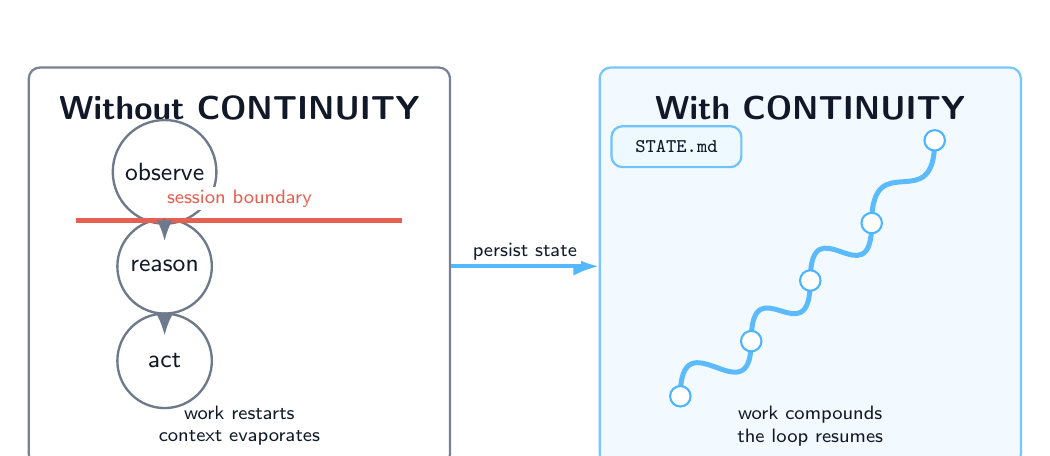
\begin{tikzpicture}[
  every node/.style={figlabel},
  panel/.style={figbox, minimum width=5.35cm, minimum height=5.05cm, align=center},
  loop/.style={draw=BitSlate!85, line width=0.85pt, circle, minimum size=1.2cm, align=center}
]
\node[panel] (left) at (0,0) {};
\node[anchor=north, figtitle, font=\sffamily\bfseries\large] at ($(left.north)+(0,-0.26)$) {Without CONTINUITY};
\foreach \y/\txt in {1.20/{observe},0.0/{reason},-1.20/{act}} {
  \node[loop] at (-0.95,\y) {\txt};
}
\draw[BitRose!90!black, line width=1.6pt] ($(left.west)+(0.62,0.58)$) -- ($(left.east)+(-0.62,0.58)$);
\node[figsmall, text=BitRose!90!black, fill=white, inner sep=1pt] at (0.0,0.86) {session boundary};
\draw[figarrow] (-0.95,0.6) -- (-0.95,0.32);
\draw[figarrow] (-0.95,-0.6) -- (-0.95,-0.88);
\node[align=center, figsmall] at (0,-2.02) {work restarts\\context evaporates};

\node[panel, fill=BitBlue!6, draw=BitBlue!65] (right) at (7.25,0) {};
\node[anchor=north, figtitle, font=\sffamily\bfseries\large] at ($(right.north)+(0,-0.26)$) {With CONTINUITY};
\draw[BitBlue!78, line width=1.8pt] ($(right.center)+(-1.65,-1.65)$)
   .. controls +(0,1.05) and +(0,-1.0) .. ($(right.center)+(-0.75,-0.95)$)
   .. controls +(0,1.0) and +(0,-1.0) .. ($(right.center)+(0.0,-0.18)$)
   .. controls +(0,1.0) and +(0,-1.0) .. ($(right.center)+(0.78,0.55)$)
   .. controls +(0,1.0) and +(0,-1.0) .. ($(right.center)+(1.58,1.6)$);
\foreach \x/\y in {-1.65/-1.65,-0.75/-0.95,0/-0.18,0.78/0.55,1.58/1.60} {
  \fill[white] ($(right.center)+(\x,\y)$) circle (0.13cm);
  \draw[BitBlue!85, line width=0.75pt] ($(right.center)+(\x,\y)$) circle (0.13cm);
}
\node[livebox, minimum width=1.65cm, minimum height=.52cm, font=\sffamily\scriptsize\bfseries] at ($(right.center)+(-1.7,1.52)$) {\statefile{STATE.md}};
\node[align=center, figsmall] at ($(right.center)+(0,-2.03)$) {work compounds\\the loop resumes};

\draw[figflow, line width=1.35pt] (left.east) -- node[above, figsmall, fill=white, inner sep=1.5pt] {persist state} (right.west);
\end{tikzpicture}
\caption{A session can end without erasing the work state. That is the core operational promise.}
\label{fig:intro-state-gap}
\end{figure}


Four kinds of state are commonly lost. First, \term{current truth} drifts: the repository may have changed, but the agent still acts on an earlier plan. Second, \term{attempt history} disappears: failures are repeated because earlier experiments were never captured. Third, \term{operational constraints} get buried in chat logs, issue threads, or a developer's head. Fourth, \term{handoff state} is weak: one agent cannot easily tell another what remains, what is blocked, and what evidence already exists.

Tool practice has started to converge on a partial fix. Codex loads \statefile{AGENTS.md} before work and composes instructions across global, repository, and directory scopes \cite{OpenAICodexAgents}. Claude Code documents persistent repository context through \file{CLAUDE.md} and distinguishes that soft context from hard enforcement \cite{AnthropicClaudeMemory,AnthropicClaudeHooks}. Hermes progressively discovers local context files as the agent moves through a project \cite{HermesContextFiles}. OpenClaw stores memory as plain Markdown on disk rather than hidden platform state \cite{OpenClawMemory}. These systems already treat the repository as part of the agent interface.

\systemname{} extends that interface into a compact state substrate. It does not ask one file to do everything. It separates stable boot guidance from mutable state, active tasks, learned lessons, append-only history, and generated evidence. The minimal core stays intentionally small:

\begin{calloutbox}[colback=BitGray,colframe=BitLine,title=Minimal CONTINUITY core]
\begin{tabularx}{\linewidth}{>{\raggedright\arraybackslash}p{2.9cm}X}
\statefile{AGENTS.md} & boot order, governance, load rules \\
\statefile{STATE.md} & current project truth \\
\statefile{TODO.md} & executable task queue \\
\statefile{LEARNINGS.md} & compact reflection and reusable lessons \\
\statefile{MEMORY.md} & durable facts index, loaded selectively \\
\file{completed/} & append-only records of finished work \\
\file{snapshots/} & recovery checkpoints \\
\file{artifacts/} & outputs, logs, test evidence \\
\statefile{CHECKPOINT.md} & approval gates for high-risk actions \\
\end{tabularx}
\end{calloutbox}

The point is not to create a repository diary. The point is to keep the smallest set of files that preserve continuity across sessions and across agents.

Recent evidence makes the design constraint sharper. Gloaguen et al. find that repository context files do not reliably improve coding-agent task success and can increase inference cost by more than 20\% on average \cite{Gloaguen2026Agents}. Dos Santos et al. report six recurring configuration smells in \statefile{AGENTS.md}-style files, including \term{context bloat} (too much irrelevant or diffuse instruction), \term{lint leakage} (tool-output noise or rules pasted directly into the manifest), \term{skill leakage} (specialized or personal instructions spilling into shared context), and \term{conflicting instructions} \cite{DosSantos2026Smells}. Those results rule out the obvious mistake: more prose is not automatically better state.

The rest of the paper develops the positive version of that negative lesson. \systemname{} works when it remains compact, scoped, current, and reviewable. The next sections show where that stance comes from, how the file grammar works, how multi-agent collaboration fits, and how the design should be evaluated and constrained.


\section{Foundations}


\begin{figure}[H]
\centering
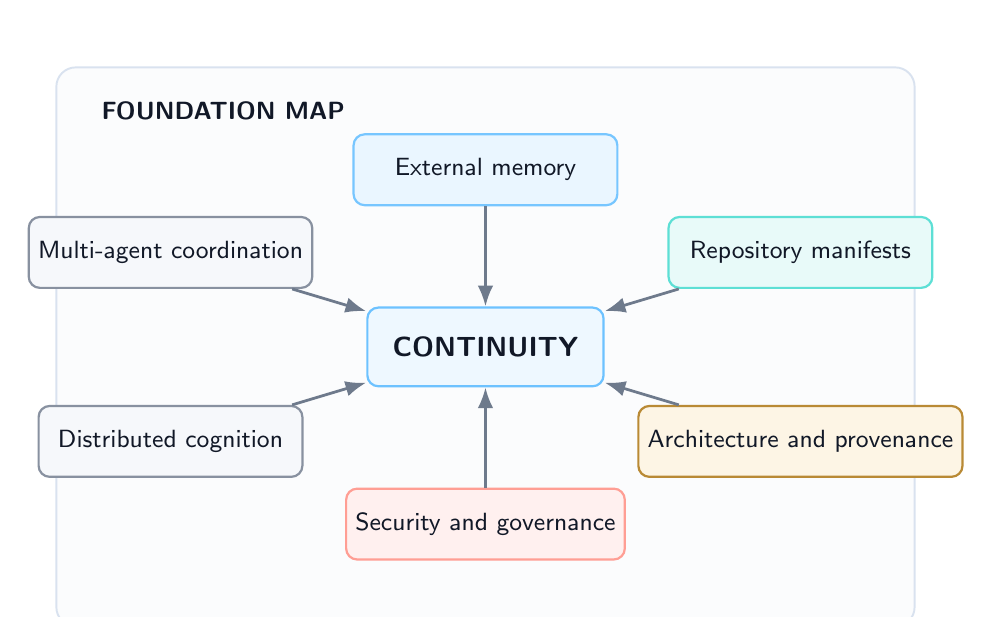
\begin{tikzpicture}[every node/.style={figlabel}, box/.style={figbox, minimum width=3.35cm, minimum height=.9cm, align=center}]
\path[figpanel] (-5.45,-3.55) rectangle (5.45,3.55);
\node[figtitle, anchor=west] at (-5.0,3.0) {FOUNDATION MAP};
\node[livebox, minimum width=3.0cm, minimum height=1.0cm, font=\sffamily\bfseries] (c) at (0,0) {CONTINUITY};
\node[box, fill=BitBlue!10, draw=BitBlue!65] (m) at (0,2.25) {External memory};
\node[box, fill=BitTeal!10, draw=BitTeal!70] (r) at (4.0,1.2) {Repository manifests};
\node[box, fill=BitGold!14, draw=BitGold!76!black] (a) at (4.0,-1.2) {Architecture and provenance};
\node[box, fill=BitRose!10, draw=BitRose!65] (g) at (0,-2.25) {Security and governance};
\node[box, fill=BitGray, draw=BitSlate!70] (d) at (-4.0,-1.2) {Distributed cognition};
\node[box, fill=BitGray, draw=BitSlate!70] (u) at (-4.0,1.2) {Multi-agent coordination};
\foreach \n in {m,r,a,g,d,u}{\draw[figarrow] (\n) -- (c);}
\end{tikzpicture}
\caption{Six literatures support the proposal. The paper sits at their intersection rather than inside only one of them.}
\label{fig:literature-map}
\end{figure}


\subsection{External memory for coding agents}


\begin{figure}[H]
\centering
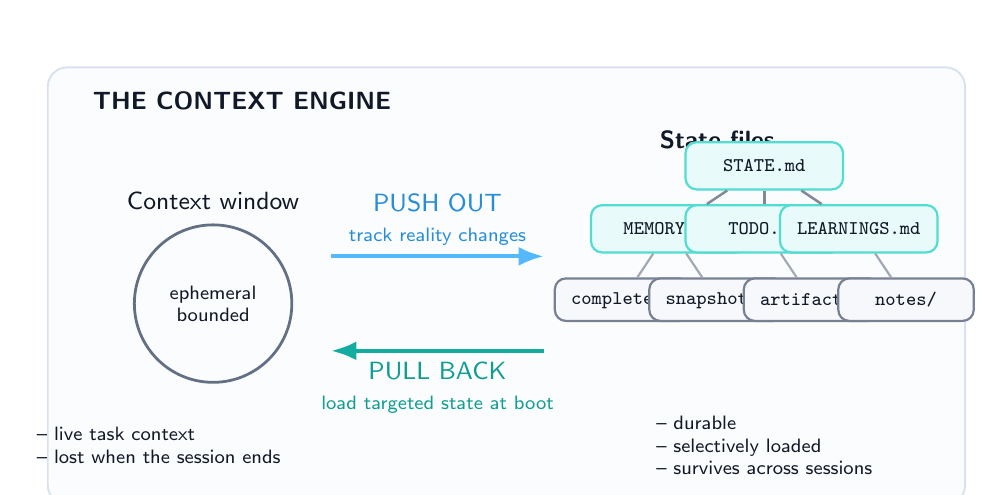
\begin{tikzpicture}[
  every node/.style={figlabel},
  file/.style={statebox, minimum width=2.0cm, minimum height=.6cm, font=\sffamily\scriptsize\bfseries, align=center},
  cold/.style={neutralbox, minimum width=1.72cm, minimum height=.54cm, font=\sffamily\scriptsize, align=center}
]
\path[figpanel] (-0.55,-2.3) rectangle (11.1,3.25);
\node[figtitle, anchor=west] at (-0.1,2.82) {THE CONTEXT ENGINE};

% left context circle
\draw[BitSlate!92, line width=1.0pt] (1.55,0.25) circle (1.0cm);
\node[align=center,font=\sffamily\small] at (1.55,1.55) {Context window};
\node[align=center,figsmall] at (1.55,0.25) {ephemeral\\bounded};
\node[align=left,figsmall] at (0.86,-1.55) {-- live task context\\-- lost when the session ends};

% middle arrows
\draw[figflow, line width=1.35pt] (3.05,0.85) -- node[above, align=center, font=\sffamily\small, text=BitBlue!82!BitNavy] {PUSH OUT\\\figsmall track reality changes} (5.75,0.85);
\draw[figreturn, line width=1.35pt] (5.75,-0.35) -- node[below, align=center, font=\sffamily\small, text=BitTeal!75!black] {PULL BACK\\\figsmall load targeted state at boot} (3.05,-0.35);

% right tree
\node[anchor=west, font=\sffamily\small\bfseries] at (7.1,2.33) {State files};
\node[file] (root) at (8.55,2.0) {\statefile{STATE.md}};
\node[file] (a1) at (7.35,1.2) {\statefile{MEMORY.md}};
\node[file] (a2) at (8.55,1.2) {\statefile{TODO.md}};
\node[file] (a3) at (9.75,1.2) {\statefile{LEARNINGS.md}};
\node[cold] (c1) at (6.75,0.3) {\file{completed/}};
\node[cold] (c2) at (7.95,0.3) {\file{snapshots/}};
\node[cold] (c3) at (9.15,0.3) {\file{artifacts/}};
\node[cold] (c4) at (10.35,0.3) {\file{notes/}};
\foreach \n in {a1,a2,a3}{\draw[BitSlate!75,line width=0.9pt] (root) -- (\n);}
\foreach \a/\b in {a1/c1,a1/c2,a2/c3,a3/c4}{\draw[BitSlate!55,line width=0.8pt] (\a) -- (\b);}
\node[align=left,figsmall] at (8.55,-1.55) {-- durable\\-- selectively loaded\\-- survives across sessions};
\end{tikzpicture}
\caption{Durable state stays outside the context window. The model only pulls back the smallest useful slice.}
\label{fig:context-engine}
\end{figure}


Modern \LLM{} systems are powerful precisely where their memory is weak. The context window is large but still finite, and tool-use traces quickly crowd out older information. That is why the memory literature repeatedly pushes state outside the model. MemGPT treats memory as a tiered system that shuttles information between active context and longer-term stores \cite{Packer2023MemGPT}. MemoryBank studies selective retention and memory updates over time \cite{Zhong2023MemoryBank}. Generative Agents and Reflexion both show that reusable behavior emerges when experience is written down, revisited, and distilled into higher-value summaries \cite{Park2023GenerativeAgents,Shinn2023Reflexion}. Survey work reaches the same conclusion: durable agent memory needs explicit write, manage, and read loops \cite{Wang2023LLMAgentSurvey}.

CONTINUITY adopts that external-memory stance but narrows the medium. It uses repository files as the persistence layer because coding agents and developers already live there.

\subsection{Repository-local manifests are already standard practice}

The repository has become part of the prompt surface. Codex, Claude Code, Hermes, and OpenClaw all expose repository-local instruction or memory files \cite{OpenAICodexAgents,AnthropicClaudeMemory,HermesContextFiles,OpenClawMemory}. CONTINUITY does not need to justify that starting point. What it adds is separation of concerns. A manifest should not double as a task log; current state should not double as an archive; and evidence should not hide inside prose.

\subsection{Architecture knowledge and workflow provenance}

Software repositories do not store code alone. They also store design intent, constraints, decisions, tradeoffs, and evidence. Classical architecture work treats those as first-class parts of the system description \cite{PerryWolf1992,Kruchten1995,TyreeAkerman2005,JansenBosch2005,ISO42010}. Empirical studies show that architecture knowledge often ends up scattered through ordinary development artifacts, including issue trackers \cite{Soliman2021AK}. Reproducibility and provenance work make the same demand from another angle: important work should be reconstructable from inputs, actions, outputs, and version history \cite{Wilson2017GoodEnough,W3CPROV,SoilandReyes2022ROCrate,Murta2014NoWorkflow}.

CONTINUITY places a lightweight state layer on top of those ideas. \statefile{STATE.md} captures what is true now. \file{completed/} and \file{artifacts/} capture what happened and what proves it.

\subsection{Coordination depends on shared artifacts}

Multi-agent work needs more than messaging. It needs a shared place where partial results, task claims, and review outcomes can be seen by others. Blackboard systems, the Contract Net Protocol, Linda tuple spaces, and the actor model all offer variants of that idea \cite{Corkill1991Blackboard,Smith1980ContractNet,Gelernter1985Linda,Hewitt1973Actor}. Recent multi-agent \LLM{} systems make the same move through role separation and explicit task exchange \cite{Wu2023AutoGen,Li2023CAMEL,Hong2023MetaGPT}. \CSCW{} and distributed cognition explain why this works: coordination improves when knowledge is externalized into inspectable artifacts \cite{Hutchins1995,Kirsh1995,Wegner1985,SchmidtSimone1996}.

CONTINUITY uses the repository as that shared surface. It is a blackboard by convention, not by runtime.

\subsection{Security limits the whole design}

Every file that enters context becomes part of the instruction boundary. Indirect prompt injection, prompt theft, and over-permissioned agent workflows all exploit that boundary \cite{Greshake2023Indirect,Liu2023HouYi,OWASPLLMTop10,SLSA}. CONTINUITY therefore treats Markdown as a soft interface. The enforcement layer lives elsewhere: hooks, schemas, permissions, tests, and review.


\section{Artifact Grammar}


\begin{figure}[H]
\centering
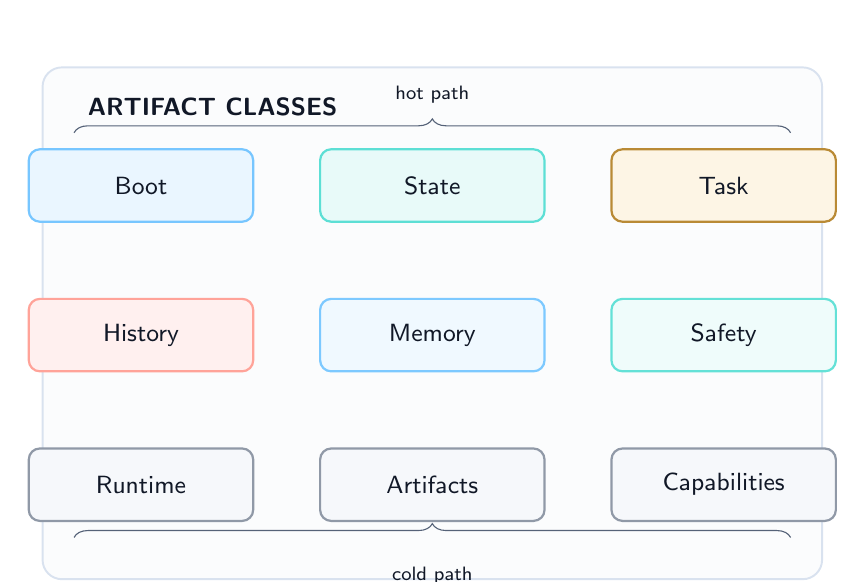
\begin{tikzpicture}[every node/.style={figlabel}, box/.style={figbox, minimum width=2.85cm, minimum height=.92cm, align=center}]
\path[figpanel] (-1.25,-3.45) rectangle (8.65,3.05);
\node[figtitle, anchor=west] at (-0.8,2.55) {ARTIFACT CLASSES};
\node[box,fill=BitBlue!10,draw=BitBlue!65] (boot) at (0,1.55) {Boot};
\node[box,fill=BitTeal!10,draw=BitTeal!70] (state) at (3.7,1.55) {State};
\node[box,fill=BitGold!14,draw=BitGold!76!black] (task) at (7.4,1.55) {Task};
\node[box,fill=BitRose!10,draw=BitRose!62] (hist) at (0,-0.35) {History};
\node[box,fill=BitBlue!7,draw=BitBlue!62] (mem) at (3.7,-0.35) {Memory};
\node[box,fill=BitTeal!7,draw=BitTeal!67] (safe) at (7.4,-0.35) {Safety};
\node[box,fill=BitGray,draw=BitSlate!65] (run) at (0,-2.25) {Runtime};
\node[box,fill=BitGray,draw=BitSlate!65] (art) at (3.7,-2.25) {Artifacts};
\node[box,fill=BitGray,draw=BitSlate!65] (cap) at (7.4,-2.25) {Capabilities};
\draw[decorate,decoration={brace,amplitude=5pt},BitSlate] (-0.85,2.22) -- (8.25,2.22) node[midway,above=7pt,figsmall] {hot path};
\draw[decorate,decoration={brace,amplitude=5pt},BitSlate] (-0.85,-2.92) -- (8.25,-2.92) node[midway,below=7pt,figsmall] {cold path};
\end{tikzpicture}
\caption{Classes are distinguished by how they load and how they change, not only by topic.}
\label{fig:grammar-ontology}
\end{figure}



\begin{figure}[H]
\centering
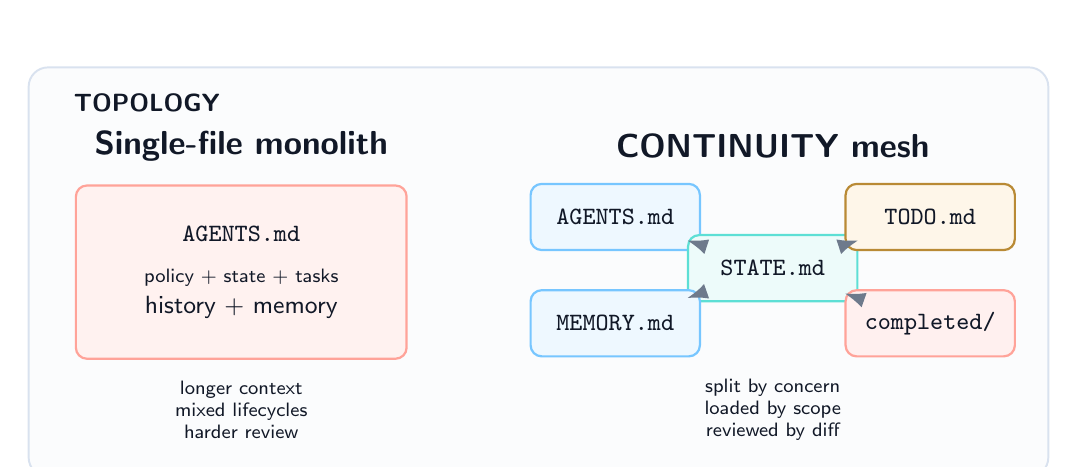
\begin{tikzpicture}[every node/.style={figlabel}, filebox/.style={figbox, align=center, minimum height=.84cm}]
\path[figpanel] (-2.7,-1.95) rectangle (10.25,3.25);
\node[figtitle, anchor=west] at (-2.25,2.8) {TOPOLOGY};
\node[font=\sffamily\bfseries\large, text=BitInk] at (0,2.25) {Single-file monolith};
\node[filebox, fill=BitRose!9, draw=BitRose!62, minimum width=4.2cm, minimum height=2.2cm] (mono) at (0,0.65) {\statefile{AGENTS.md}\\[4pt]\figsmall policy + state + tasks\\history + memory};
\node[align=center, figsmall] at (0,-1.1) {longer context\\mixed lifecycles\\harder review};

\node[font=\sffamily\bfseries\large, text=BitInk] at (6.75,2.25) {CONTINUITY mesh};
\node[filebox, fill=BitBlue!8, draw=BitBlue!65, minimum width=2.15cm] (a) at (4.75,1.35) {\statefile{AGENTS.md}};
\node[filebox, fill=BitTeal!8, draw=BitTeal!70, minimum width=2.15cm] (s) at (6.75,0.7) {\statefile{STATE.md}};
\node[filebox, fill=BitGold!12, draw=BitGold!76!black, minimum width=2.15cm] (t) at (8.75,1.35) {\statefile{TODO.md}};
\node[filebox, fill=BitBlue!8, draw=BitBlue!65, minimum width=2.15cm] (m) at (4.75,0.0) {\statefile{MEMORY.md}};
\node[filebox, fill=BitRose!10, draw=BitRose!62, minimum width=2.15cm] (h) at (8.75,0.0) {\file{completed/}};
\draw[figarrow] (a) -- (s);
\draw[figarrow] (t) -- (s);
\draw[figarrow] (s) -- (h);
\draw[figarrow] (m) -- (s);
\node[align=center, figsmall] at (6.75,-1.1) {split by concern\\loaded by scope\\reviewed by diff};
\end{tikzpicture}
\caption{The mesh preserves separate lifecycles instead of forcing all agent context into one manifest.}
\label{fig:monolith-mesh}
\end{figure}


CONTINUITY organizes repository artifacts into classes with different mutability and load rules. That distinction matters. When current state, historical notes, and reusable knowledge collapse into the same file, the result is usually drift or bloat. In this paper, upper-case filenames such as \statefile{STATE.md} denote the live state layer, while lower-case paths such as \file{completed/} and \file{artifacts/} denote history or evidence stores.


\begin{table}[H]
\centering
\caption{CONTINUITY artifact classes. The key distinction is between what loads by default and what stays cold until needed.}
\label{tab:file-taxonomy}
\small
\rowcolors{2}{BitGray}{white}
\begin{tabularx}{\linewidth}{>{\raggedright\arraybackslash}p{1.55cm}>{\raggedright\arraybackslash}p{3.05cm}>{\raggedright\arraybackslash}p{1.9cm}>{\raggedright\arraybackslash}p{1.75cm}X}
\rowcolor{BitNavy!8}
\textbf{Class} & \textbf{Examples} & \textbf{Mutability} & \textbf{Default load} & \textbf{Function} \\
Boot & \statefile{AGENTS.md}, \statefile{BOOT.md} & rare edits & yes & startup logic, norms, governance \\
State & \statefile{STATE.md}, \statefile{CONTEXT.md} & overwrite & scoped & current project truth \\
Task & \statefile{TODO.md}, \statefile{TASKS.md} & frequent & scoped & executable queue and ownership \\
Memory & \statefile{MEMORY.md}, \statefile{LEARNINGS.md} & curated & selective & durable facts and distilled lessons \\
History & \file{completed/}, \file{snapshots/} & append-only & no & evidence and prior states \\
Safety & \statefile{CHECKPOINT.md}, \statefile{WARNING.md} & stable & yes & approvals and hazard notes \\
Runtime & \file{claims/}, \file{runs/} & structured & per run & activity trace and coordination \\
Artifacts & \file{artifacts/}, \file{reviews/} & append or curated & no & logs, plots, outputs, review records \\
\end{tabularx}
\end{table}


\subsection{Core terms}

\begin{description}[leftmargin=2.6cm,style=nextline]
  \item[Repository-native state] Project state stored inside the repository rather than inside hidden platform memory.
  \item[Current truth] The smallest accurate description of what is true right now.
  \item[State reconciliation] Updating state artifacts after code, tests, or decisions change.
  \item[Scoped loading] Resolving only the manifest, state, and task files relevant to the current path.
  \item[Semantic history] Append-only records organized by meaning: completed work, reviews, evidence, and snapshots.
  \item[Soft constraint] A model-visible instruction that is not technically enforced.
  \item[Hard constraint] A rule enforced by hooks, tests, permissions, schemas, or human approval.
\end{description}

\subsection{Minimal core versus template library}

The paper defends a \term{minimal reference core}, not the largest possible template set. A repository that only needs \statefile{AGENTS.md}, \statefile{STATE.md}, and \statefile{TODO.md} should not be pressured into creating ten more files. The extended topology is valuable as a library of patterns. It is not a proof that every pattern should be loaded.


\begin{figure}[H]
\centering
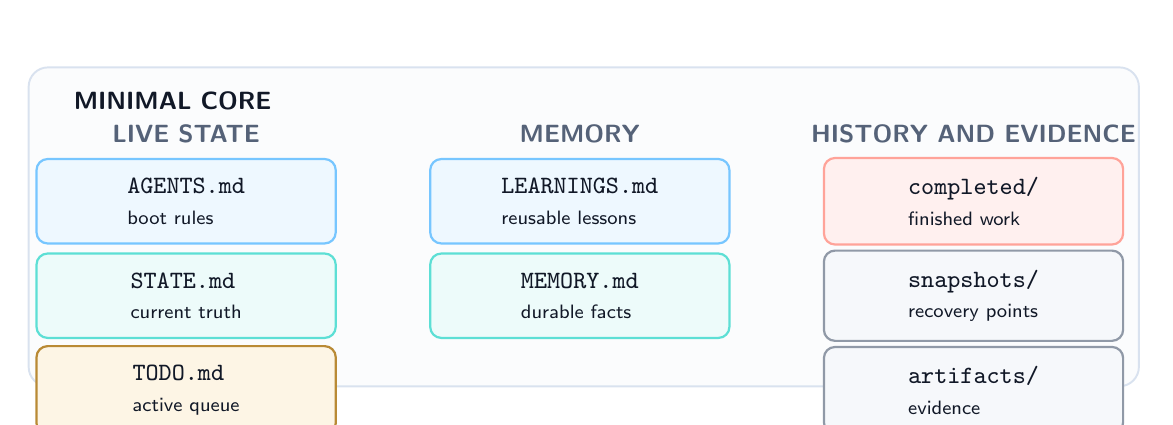
\begin{tikzpicture}[every node/.style={figlabel}, box/.style={figbox, align=left, minimum width=3.8cm, minimum height=.88cm, inner sep=7pt}]
\path[figpanel] (-2.0,-0.95) rectangle (12.1,3.1);
\node[figtitle, anchor=west] at (-1.55,2.68) {MINIMAL CORE};
\node[font=\sffamily\bfseries\small, text=BitSlate] at (0,2.25) {LIVE STATE};
\node[font=\sffamily\bfseries\small, text=BitSlate] at (5.0,2.25) {MEMORY};
\node[font=\sffamily\bfseries\small, text=BitSlate] at (10.0,2.25) {HISTORY AND EVIDENCE};

\node[box, fill=BitBlue!8, draw=BitBlue!65] at (0,1.4) {\statefile{AGENTS.md}\\\figsmall boot rules};
\node[box, fill=BitTeal!8, draw=BitTeal!70] at (0,0.2) {\statefile{STATE.md}\\\figsmall current truth};
\node[box, fill=BitGold!14, draw=BitGold!76!black] at (0,-1.0) {\statefile{TODO.md}\\\figsmall active queue};
\node[box, fill=BitBlue!8, draw=BitBlue!65] at (5.0,1.4) {\statefile{LEARNINGS.md}\\\figsmall reusable lessons};
\node[box, fill=BitTeal!8, draw=BitTeal!70] at (5.0,0.2) {\statefile{MEMORY.md}\\\figsmall durable facts};
\node[box, fill=BitRose!10, draw=BitRose!62] at (10.0,1.4) {\file{completed/}\\\figsmall finished work};
\node[box, fill=BitGray, draw=BitSlate!65] at (10.0,0.2) {\file{snapshots/}\\\figsmall recovery points};
\node[box, fill=BitGray, draw=BitSlate!65] at (10.0,-1.0) {\file{artifacts/}\\\figsmall evidence};
\end{tikzpicture}
\caption{The minimal core separates live state from archival material. Upper-case filenames denote the live state files.}
\label{fig:minimal-core}
\end{figure}


\subsection{State, history, and knowledge are different objects}

Current state is overwritten. History accumulates. Knowledge is distilled. The operational grammar depends on keeping those three objects separate.


\begin{figure}[H]
\centering
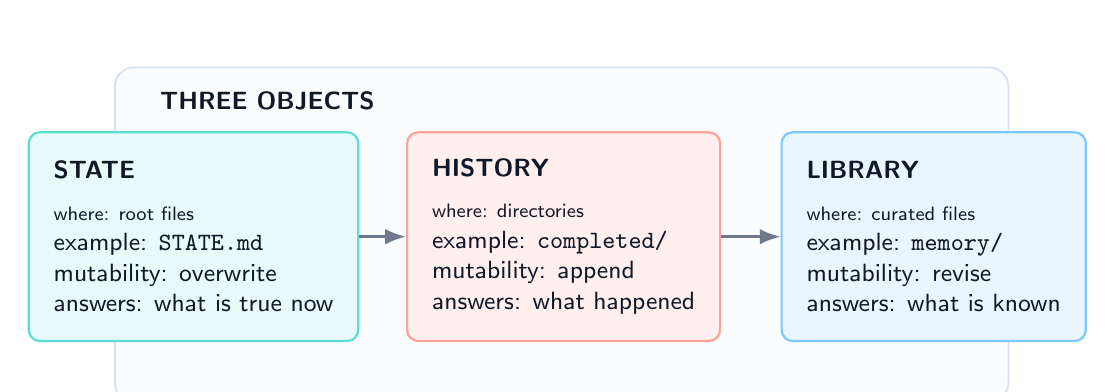
\begin{tikzpicture}[every node/.style={figlabel}, card/.style={figbox, minimum width=3.55cm, minimum height=2.65cm, align=left, inner sep=9pt}]
\path[figpanel] (-1.0,-2.1) rectangle (10.35,2.15);
\node[figtitle, anchor=west] at (-0.55,1.72) {THREE OBJECTS};
\node[card, fill=BitTeal!10, draw=BitTeal!72] (state) at (0,0) {\textbf{STATE}\\[4pt]\figsmall where: root files\\example: \statefile{STATE.md}\\mutability: overwrite\\answers: what is true now};
\node[card, fill=BitRose!10, draw=BitRose!62] (hist) at (4.7,0) {\textbf{HISTORY}\\[4pt]\figsmall where: directories\\example: \file{completed/}\\mutability: append\\answers: what happened};
\node[card, fill=BitBlue!10, draw=BitBlue!62] (lib) at (9.4,0) {\textbf{LIBRARY}\\[4pt]\figsmall where: curated files\\example: \file{memory/}\\mutability: revise\\answers: what is known};
\draw[figarrow] (state.east) -- (hist.west);
\draw[figarrow] (hist.east) -- (lib.west);
\end{tikzpicture}
\caption{Current truth, history, and reusable knowledge should not collapse into one file.}
\label{fig:state-history-knowledge}
\end{figure}



\section{Operational Model}


\begin{figure}[H]
\centering
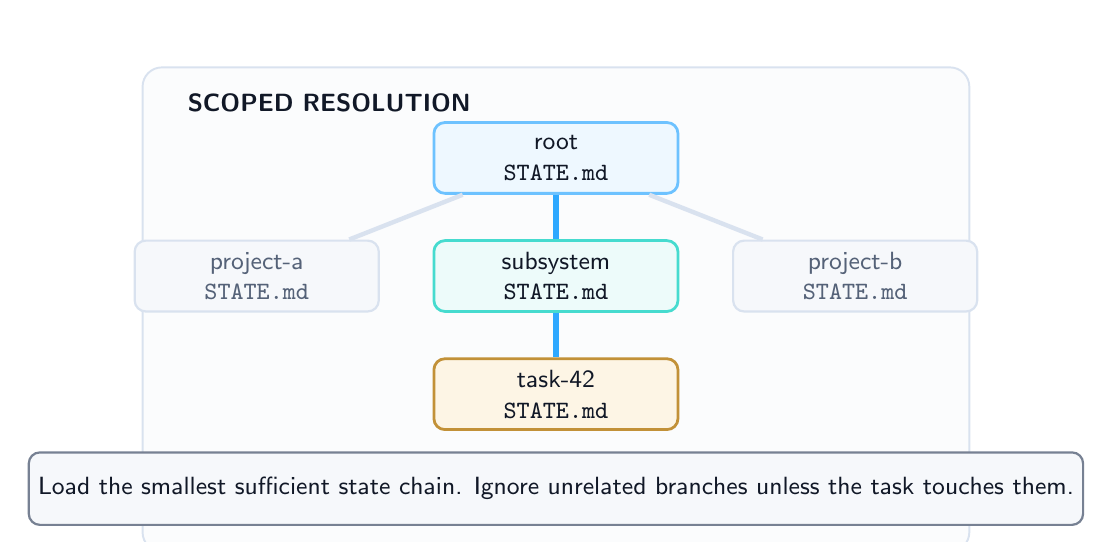
\begin{tikzpicture}[every node/.style={figlabel}, box/.style={figbox, minimum width=3.1cm, minimum height=.9cm, align=center}]
\path[figpanel] (-1.25,-3.15) rectangle (9.25,3.0);
\node[figtitle, anchor=west] at (-0.8,2.55) {SCOPED RESOLUTION};
\node[box, fill=BitBlue!8, draw=BitBlue!70, line width=1.0pt] (root) at (4,1.85) {root\\\statefile{STATE.md}};
\node[box, fill=BitGray, draw=BitLine, text=BitSlate] (pa) at (0.2,0.35) {project-a\\\statefile{STATE.md}};
\node[box, fill=BitTeal!8, draw=BitTeal!80, line width=1.0pt] (sub) at (4,0.35) {subsystem\\\statefile{STATE.md}};
\node[box, fill=BitGray, draw=BitLine, text=BitSlate] (pb) at (7.8,0.35) {project-b\\\statefile{STATE.md}};
\node[box, fill=BitGold!14, draw=BitGold!80!black, line width=1.0pt] (task) at (4,-1.15) {task-42\\\statefile{STATE.md}};
\draw[BitLine,line width=1.6pt] (root) -- (pa);
\draw[BitLine,line width=1.6pt] (root) -- (pb);
\draw[BitBlue,line width=2.0pt] (root) -- (sub) -- (task);
\node[neutralbox, minimum width=8.4cm, minimum height=.92cm, align=center] at (4,-2.35) {Load the smallest sufficient state chain. Ignore unrelated branches unless the task touches them.};
\end{tikzpicture}
\caption{Scoped resolution follows the active branch and leaves unrelated repository state cold.}
\label{fig:scope-resolution}
\end{figure}


A Continuity workspace can be modeled as a tuple
\begin{equation}
\label{eq:workspace}
C = \langle M, S, T, L, H, A, G, V, \Omega \rangle,
\end{equation}
where $M$ is the manifest set, $S$ the current-state set, $T$ the task queue, $L$ learned memory, $H$ semantic history, $A$ generated artifacts, $G$ version history, $V$ validators and enforcement mechanisms, and $\Omega$ the active agent set.

For a path $p$ and context budget $B$, Continuity does not load every available file. It loads the smallest relevant slice:
\begin{equation}
\label{eq:load}
load(p,B)=\operatorname{select}(M\cup S\cup T\cup L\mid scope(p)) \quad \text{s.t.} \quad tokens(load)\leq B.
\end{equation}
The function is intentionally abstract. Its purpose is normative, not implementation-specific: keep the live context small, task-specific, and explicit.

\subsection{Reconciliation invariant}

Every action that changes repository reality risks invalidating recorded state. Continuity therefore requires a reconciliation step after meaningful work:
\begin{equation}
\label{eq:reconcile}
state(C_{after}) \approx reality(R_{after}).
\end{equation}
The approximation symbol is deliberate. Natural-language state files cannot perfectly encode repository truth. They can, however, remain close enough to prevent stale planning and repeated errors.


\begin{figure}[H]
\centering
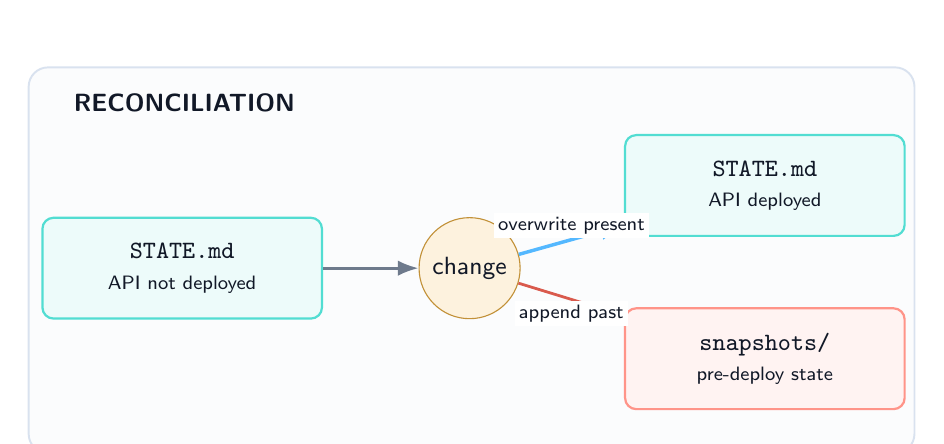
\begin{tikzpicture}[every node/.style={figlabel}, file/.style={figbox, minimum width=3.55cm, minimum height=1.28cm, align=center}]
\path[figpanel] (-1.05,-2.35) rectangle (10.2,2.55);
\node[figtitle, anchor=west] at (-0.6,2.1) {RECONCILIATION};
\node[file, fill=BitTeal!8, draw=BitTeal!75] (old) at (0.9,0) {\statefile{STATE.md}\\\figsmall API not deployed};
\node[draw, circle, fill=BitGold!18, draw=BitGold!80!black, minimum size=1.28cm, font=\sffamily\small] (change) at (4.55,0) {change};
\node[file, fill=BitTeal!8, draw=BitTeal!75] (new) at (8.3,1.05) {\statefile{STATE.md}\\\figsmall API deployed};
\node[file, fill=BitRose!8, draw=BitRose!72] (hist) at (8.3,-1.15) {\file{snapshots/}\\\figsmall pre-deploy state};
\draw[figarrow] (old) -- (change);
\draw[figflow] (change) -- node[above, figsmall, fill=white, inner sep=1.5pt] {overwrite present} (new);
\draw[figdanger] (change) -- node[below, figsmall, fill=white, inner sep=1.5pt] {append past} (hist);
\end{tikzpicture}
\caption{The live state updates in place, while the old state moves to append-only history.}
\label{fig:reconciliation-loop}
\end{figure}


\subsection{Safety inheritance}

Local context should refine parent guidance, not weaken it. If a repository-level file forbids destructive commands without approval, a subdirectory file must not silently remove that rule. Continuity expresses that constraint as
\begin{equation}
\label{eq:safety}
safety(child) \supseteq safety(parent).
\end{equation}

\subsection{Evidence requirement}

Completion without evidence is only an assertion. Continuity therefore treats a task as complete only when a reviewable artifact exists:
\begin{equation}
\label{eq:evidence}
status(task)=complete \Rightarrow \exists e\in(A\cup G\cup H): supports(e,task).
\end{equation}
A passing test log, an artifact bundle, a review record, or a commit can satisfy this condition.


\section{Negative Evidence and Design Constraints}


\begin{figure}[H]
\centering
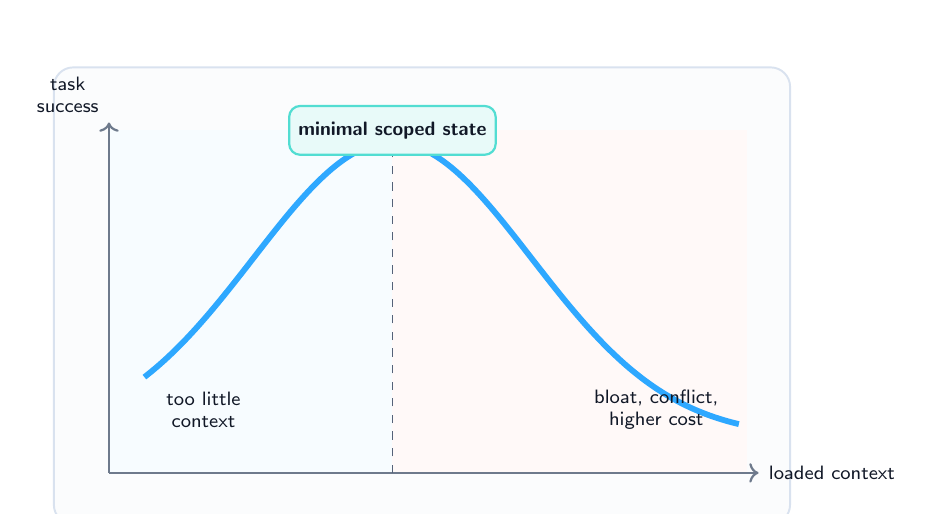
\begin{tikzpicture}[every node/.style={figlabel}]
\path[figpanel] (-0.7,-0.65) rectangle (8.65,5.15);
\fill[BitBlue!4] (0,0) rectangle (3.6,4.35);
\fill[BitRose!4] (3.6,0) rectangle (8.1,4.35);
\draw[->, thick, BitSlate!85] (0,0) -- (8.25,0) node[right, figsmall] {loaded context};
\draw[->, thick, BitSlate!85] (0,0) -- (0,4.45) node[above left, align=center, figsmall] {task\\success};
\draw[BitBlue, line width=2.1pt, domain=.45:8.0, samples=90, smooth] plot (\x,{3.75*exp(-0.16*(\x-3.6)*(\x-3.6))+0.45});
\draw[dashed, BitSlate] (3.6,0) -- (3.6,4.05);
\node[statebox, minimum width=2.35cm, minimum height=.62cm, font=\sffamily\scriptsize\bfseries] at (3.6,4.35) {minimal scoped state};
\node[align=center, figsmall] at (1.2,0.8) {too little\\context};
\node[align=center, figsmall] at (6.95,0.8) {bloat, conflict,\\higher cost};
\end{tikzpicture}
\caption{The design hypothesis is an inverted U: some state helps, but unscoped context becomes harmful.}
\label{fig:constraint-funnel}
\end{figure}

The most useful recent papers in this area are cautionary. Gloaguen et al. show that repository-level context files do not automatically improve coding-agent performance and can increase inference cost substantially \cite{Gloaguen2026Agents}. Dos Santos et al. show that context files themselves suffer from recurring maintenance defects \cite{DosSantos2026Smells}. CONTINUITY treats those findings as hard design pressure, not as footnotes.


\begin{table}[H]
\centering
\caption{Recent negative evidence translated into design constraints.}
\label{tab:negative-constraints}
\footnotesize
\rowcolors{2}{BitGray}{white}
\begin{tabularx}{\linewidth}{>{\raggedright\arraybackslash}p{2.15cm}>{\raggedright\arraybackslash}p{4.35cm}X}
\rowcolor{BitNavy!8}
\textbf{Observed risk} & \textbf{Practical meaning} & \textbf{CONTINUITY response} \\
Context bloat & too much low-signal text enters the live prompt & root budgets, scoped loading, archives off the hot path \\
Conflicting instructions & multiple files tell the agent incompatible things & lints, review, parent-child safety checks \\
Stale state & current files lag behind repository reality & post-action reconciliation and freshness checks \\
False completion & tasks marked done without proof & artifact requirement and review links \\
Soft policy failure & prose alone cannot enforce critical rules & hooks, tests, permissions, sandboxing \\
Generated noise & LLM-written summaries become canonical too early & promotion only after review \\
Multi-agent collision & overlapping edits create duplicate or inconsistent work & claims, branch isolation, merge checks \\
\end{tabularx}
\end{table}


\subsection{Anti-patterns}

\sectionlead{Manifest monolith.} One giant file tries to store policy, current state, old history, and tutorial prose. The result is noise.

\sectionlead{State diary.} \statefile{STATE.md} becomes a chronological log instead of a compact statement of current truth.

\sectionlead{Archive-on-boot.} Old snapshots and completed work load by default, wasting context budget.

\sectionlead{False completion.} Tasks move to done without tests, artifacts, or reviewable evidence.

\sectionlead{Unbounded local override.} A nested file quietly weakens a repository-level safety rule.

Each anti-pattern has the same cure: keep state narrow, move history out of the hot path, and enforce what prose alone cannot enforce.


\section{Implementation Blueprint}


\begin{figure}[H]
\centering
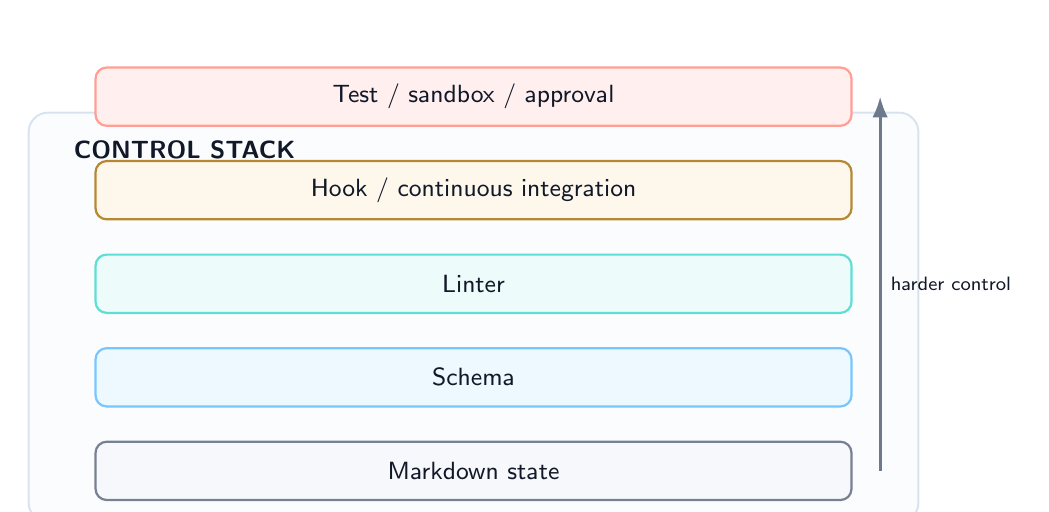
\begin{tikzpicture}[node distance=0.42cm, every node/.style={figlabel}, layer/.style={figbox, minimum width=9.6cm, minimum height=.74cm, align=center}]
\path[figpanel] (-0.85,-0.65) rectangle (10.45,4.55);
\node[figtitle, anchor=west] at (-0.4,4.08) {CONTROL STACK};
\node[layer, fill=BitGray] (p) at (4.8,0) {Markdown state};
\node[layer, above=of p, fill=BitBlue!8, draw=BitBlue!65] (s) {Schema};
\node[layer, above=of s, fill=BitTeal!8, draw=BitTeal!70] (l) {Linter};
\node[layer, above=of l, fill=BitGold!10, draw=BitGold!75!black] (h) {Hook / continuous integration};
\node[layer, above=of h, fill=BitRose!10, draw=BitRose!65] (t) {Test / sandbox / approval};
\draw[figarrow] ($(p.east)+(0.35,0)$) -- node[right, figsmall] {harder control} ($(t.east)+(0.35,0)$);
\end{tikzpicture}
\caption{Readable text is useful. Reliable control requires stronger layers around it.}
\label{fig:enforcement-stack}
\end{figure}


A practical Continuity implementation has two layers. The first layer is human-readable Markdown or YAML front matter. The second layer is deterministic validation.

\subsection{Example file header}

\begin{lstlisting}
---
continuity_type: state
scope: repository
loads_on: boot
mutability: overwrite-current
updates_after:
  - architecture_change
  - task_completion
  - failed_assumption
validation:
  - max_lines: 180
  - no_unresolved_placeholders
  - no_conflicting_status
---
\end{lstlisting}

\subsection{Hooks and validators}

A useful implementation should provide at least five checks.
\begin{enumerate}
  \item \textbf{Pre-load budget checks} stop archive files or oversized manifests from loading by default.
  \item \textbf{Pre-action scope checks} verify that the agent has loaded the nearest relevant state chain.
  \item \textbf{Post-action reconciliation checks} flag when code changed but \statefile{STATE.md} or \statefile{TODO.md} did not.
  \item \textbf{Artifact checks} reject task completion without evidence links, test output, or commits.
  \item \textbf{Safety checks} detect nested files that weaken parent safety rules.
\end{enumerate}

\subsection{Promotion rules}

Generated state should not become canonical automatically. A run summary written by an agent can seed \file{LEARNINGS.md} or \file{completed/}, but promotion into \statefile{STATE.md} or repository-wide memory should pass through review, linting, and freshness checks.

\subsection{Why this layer matters}

The implementation layer prevents the central category error of the whole topic: confusing readable text with reliable control. Continuity is strongest when the repository shows the state and the surrounding tooling checks that the state still makes sense.


\section{Multi-Agent Collaboration}


\begin{figure}[H]
\centering
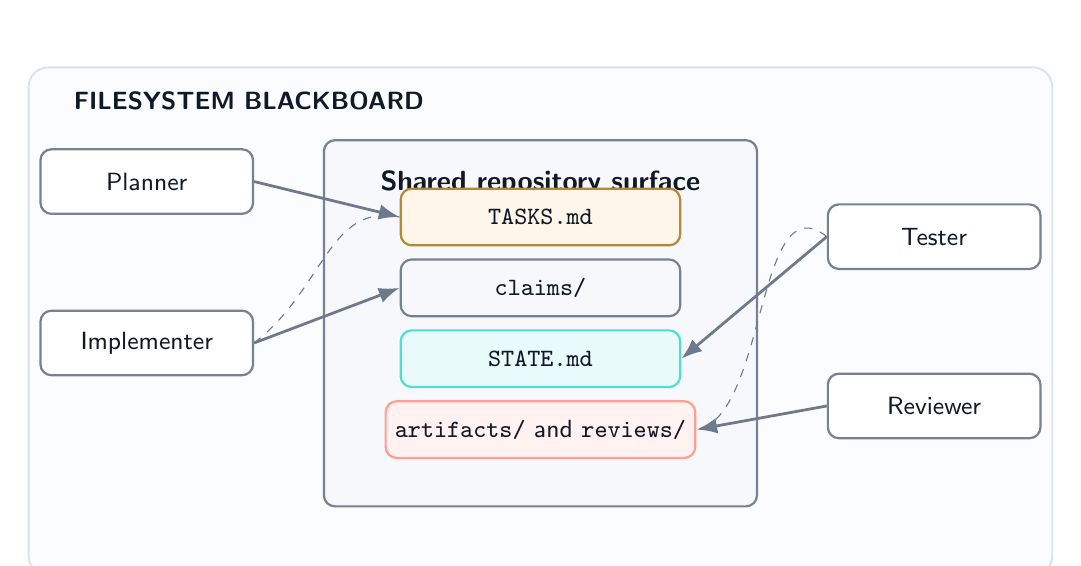
\begin{tikzpicture}[every node/.style={figlabel}, agent/.style={figbox, minimum width=2.7cm, minimum height=.82cm, align=center}]
\path[figpanel] (-6.5,-3.3) rectangle (6.5,3.15);
\node[figtitle, anchor=west] at (-6.05,2.72) {FILESYSTEM BLACKBOARD};
\node[neutralbox, minimum width=5.5cm, minimum height=4.65cm] (board) at (0,-0.1) {};
\node[anchor=north, font=\sffamily\bfseries\normalsize] at ($(board.north)+(0,-0.28)$) {Shared repository surface};
\node[taskbox, minimum width=3.55cm, minimum height=.72cm] (tasks) at (0,1.25) {\statefile{TASKS.md}};
\node[neutralbox, minimum width=3.55cm, minimum height=.72cm] (claims) at (0,0.35) {\file{claims/}};
\node[statebox, minimum width=3.55cm, minimum height=.72cm] (state) at (0,-0.55) {\statefile{STATE.md}};
\node[histbox, minimum width=3.55cm, minimum height=.72cm] (art) at (0,-1.45) {\file{artifacts/} and \file{reviews/}};

\node[agent] (planner) at (-5.0,1.7) {Planner};
\node[agent] (impl) at (-5.0,-0.35) {Implementer};
\node[agent] (tester) at (5.0,1.0) {Tester};
\node[agent] (reviewer) at (5.0,-1.15) {Reviewer};
\draw[figarrow] (planner.east) -- (tasks.west);
\draw[figarrow] (impl.east) -- (claims.west);
\draw[figarrow] (tester.west) -- (state.east);
\draw[figarrow] (reviewer.west) -- (art.east);
\draw[dashed, BitSlate!85] (impl.east) .. controls +(.9,.7) and +(-.9,.18) .. (tasks.west);
\draw[dashed, BitSlate!85] (tester.west) .. controls +(-.9,.72) and +(.9,.15) .. (art.east);
\end{tikzpicture}
\caption{Agents coordinate through a shared file surface. Locks, permissions, and scheduling still live outside the files themselves.}
\label{fig:multi-agent-blackboard}
\end{figure}


CONTINUITY becomes more useful when several agents or humans share the same repository, but multi-agent use also raises the cost of ambiguity. A shared \statefile{TASKS.md} is helpful only if agents can claim work, avoid overlap, and leave handoff evidence behind.

\subsection{Repository as filesystem blackboard}

The shared repository can play the role of a versioned blackboard. Agents read the active queue, claim a task, load the relevant state slice, execute work on a branch, publish evidence, and request review. That pattern aligns with blackboard coordination and contract-based allocation without pretending that the repository itself is a scheduler \cite{Corkill1991Blackboard,Smith1980ContractNet}.

\subsection{Minimal collaboration artifacts}

A workable multi-agent setup needs only a few extra artifacts:
\begin{itemize}
  \item \statefile{TASKS.md} for the queue,
  \item \file{claims/} for task ownership and expiry,
  \item \file{BINDING.schema.json} for role or permission contracts,
  \item \file{artifacts/} for outputs and test evidence,
  \item \file{reviews/} for approval and merge decisions.
\end{itemize}

\subsection{Collision control}

Two agents should not edit the same semantic object without coordination. In practice that means branch isolation, expiring claims, merge checks, and review gates. CONTINUITY can record these controls, but external tooling must enforce them.

\subsection{Handoff quality}

The main win is not full autonomy. The main win is cleaner handoff. When an implementer agent stops, the tester or reviewer should be able to answer three questions immediately: what changed, what remains, and what proves the current state.


\section{Evaluation Agenda}


\begin{figure}[H]
\centering
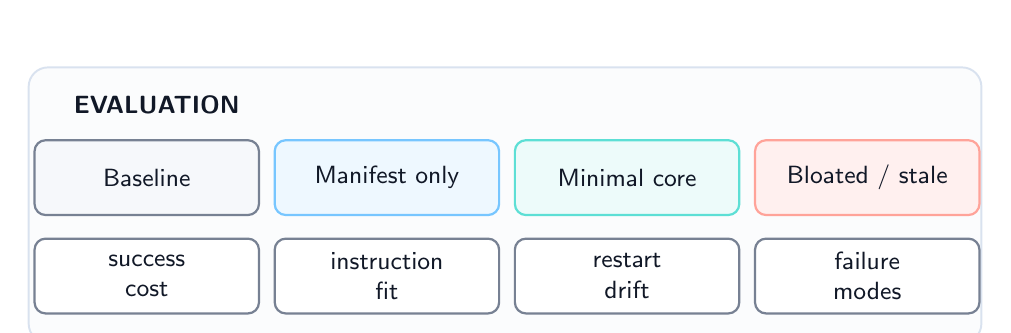
\begin{tikzpicture}[every node/.style={figlabel,align=center}, cell/.style={figbox, minimum width=2.85cm, minimum height=.95cm}]
\path[figpanel] (-1.1,-0.95) rectangle (11.0,2.55);
\node[figtitle, anchor=west] at (-0.65,2.08) {EVALUATION};
\node[cell, fill=BitGray] at (0.4,1.15) {Baseline};
\node[cell, fill=BitBlue!8, draw=BitBlue!65] at (3.45,1.15) {Manifest only};
\node[cell, fill=BitTeal!8, draw=BitTeal!70] at (6.5,1.15) {Minimal core};
\node[cell, fill=BitRose!10, draw=BitRose!62] at (9.55,1.15) {Bloated / stale};
\node[cell] at (0.4,-0.1) {success\\cost};
\node[cell] at (3.45,-0.1) {instruction\\fit};
\node[cell] at (6.5,-0.1) {restart\\drift};
\node[cell] at (9.55,-0.1) {failure\\modes};
\end{tikzpicture}
\caption{The evaluation should compare useful state, no state, and harmful state.}
\label{fig:evaluation-matrix}
\end{figure}


The right evaluation target is not "does any context file help?" The right target is narrower: under what conditions does a compact, validated state layer improve repository work, and when does it become overhead?

\subsection{Conditions}

The core conditions are baseline (no repository state), manifest-only, minimal Continuity, minimal Continuity with hooks, full topology, and failure modes such as stale state, bloated context, and conflicting local instructions.

\subsection{Benchmarks and tasks}

Existing repository benchmarks such as \SWEbench{} remain useful for patch correctness \cite{Jimenez2024SWEbench}. They do not, however, measure resumption, repeated-error avoidance, or multi-agent collision. CONTINUITY therefore needs a custom task family with interruptions, stale-state traps, cross-branch handoffs, and malicious or noisy context.

\subsection{Metrics}


\begin{table}[H]
\centering
\caption{Primary metric families for a CONTINUITY evaluation.}
\label{tab:evaluation-metrics}
\small
\rowcolors{2}{BitGray}{white}
\begin{tabularx}{\linewidth}{>{\raggedright\arraybackslash}p{2.9cm}X}
\rowcolor{BitNavy!8}
\textbf{Metric family} & \textbf{Examples} \\
Task outcome & success rate, pass@1, regression count, patch correctness \\
Efficiency & input tokens, output tokens, tool calls, wall-clock time, cost \\
Continuity & resumption latency, repeated-error rate, stale-state incidence, reconciliation completeness \\
Multi-agent & claim conflict rate, duplicate work, merge conflicts, handoff success \\
Governance & instruction compliance, review time, smell prevalence, override frequency \\
Security & prompt-injection obedience, secret leakage, unauthorized action attempts \\
\end{tabularx}
\end{table}


The most interesting metrics are often not the headline ones. Task success matters, but so do resumption latency, repeated-error rate, evidence completeness, human review time, and collision frequency.

\subsection{Ablations}

Ablations should remove \statefile{STATE.md}, \statefile{TODO.md}, \statefile{LEARNINGS.md}, scoped loading, evidence requirements, and validation hooks. Additional ablations should intentionally inject context bloat, stale facts, and local instruction conflicts.

\subsection{Expected shape of the results}

The expected positive result is modest: faster restarts, better handoff, cleaner audit trails, and fewer repeated failures. The expected negative result is equally important: larger context topologies should cost more and may perform worse. A credible paper should publish both.


\section{Threat Model}


\begin{figure}[H]
\centering
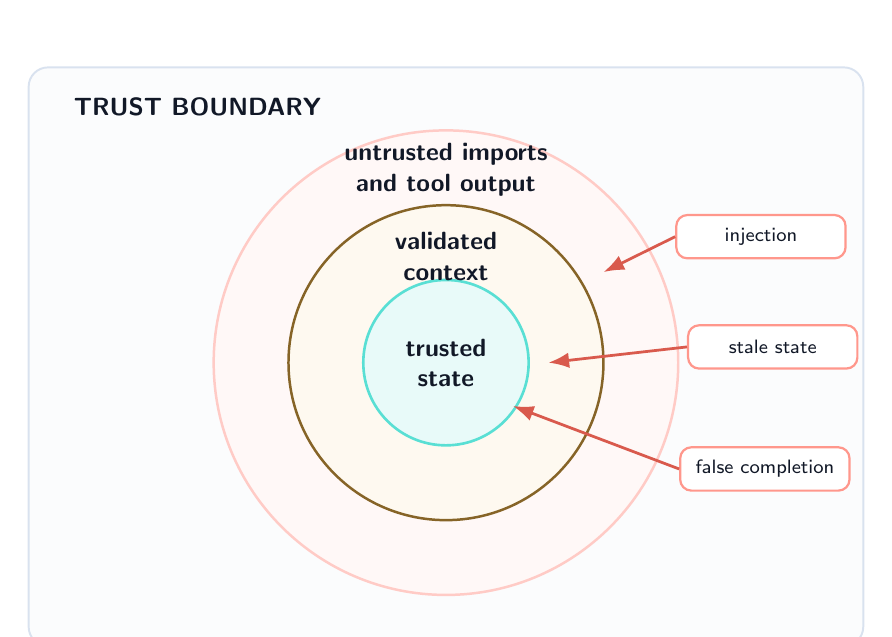
\begin{tikzpicture}[every node/.style={figlabel}]
\path[figpanel] (-5.3,-3.6) rectangle (5.3,3.75);
\node[figtitle, anchor=west] at (-4.85,3.25) {TRUST BOUNDARY};
\fill[BitRose!5] (0,0) circle (2.95cm);
\draw[BitRose!35,line width=0.9pt] (0,0) circle (2.95cm);
\fill[BitGold!8] (0,0) circle (2.0cm);
\draw[BitGold!55!black,line width=0.9pt] (0,0) circle (2.0cm);
\fill[BitTeal!10] (0,0) circle (1.05cm);
\draw[BitTeal!72,line width=0.95pt] (0,0) circle (1.05cm);
\node[align=center,font=\sffamily\small\bfseries] at (0,2.45) {untrusted imports\\and tool output};
\node[align=center,font=\sffamily\small\bfseries] at (0,1.35) {validated\\context};
\node[align=center,font=\sffamily\small\bfseries] at (0,0) {trusted\\state};
\node[histbox, fill=white, draw=BitRose!70, minimum width=2.15cm, minimum height=.55cm, font=\sffamily\scriptsize] (inj) at (4.0,1.6) {injection};
\node[histbox, fill=white, draw=BitRose!70, minimum width=2.15cm, minimum height=.55cm, font=\sffamily\scriptsize] (stale) at (4.15,0.2) {stale state};
\node[histbox, fill=white, draw=BitRose!70, minimum width=2.15cm, minimum height=.55cm, font=\sffamily\scriptsize] (falsec) at (4.05,-1.35) {false completion};
\draw[figdanger] (inj.west) -- (2.0,1.15);
\draw[figdanger] (stale.west) -- (1.3,0.0);
\draw[figdanger] (falsec.west) -- (.85,-.55);
\end{tikzpicture}
\caption{Trust rises only after validation. Raw repository text is not automatically safe context.}
\label{fig:threat-surface}
\end{figure}


Continuity moves useful state into plain files. That improves visibility, but it also creates an obvious attack surface.

\subsection{Assets}

The protected assets are source code, secrets, project state, task queues, branch and review records, generated artifacts, and tool permissions.

\subsection{Adversaries}

Relevant adversaries include malicious pull requests, poisoned issue bodies, compromised documentation, prompt-injected tool output, careless agents, stale generated summaries, and over-permissioned automation.

\subsection{Failure modes}

The core failures are prompt injection, silent instruction override, stale-state obedience, false completion, secret persistence, and agent collision. Multi-agent use adds lock poisoning, fake claims, and adversarial handoff records.

\subsection{Mitigations}


\begin{table}[H]
\centering
\caption{Condensed threat model.}
\label{tab:threat-model}
\small
\rowcolors{2}{BitGray}{white}
\begin{tabularx}{\linewidth}{>{\raggedright\arraybackslash}p{2.75cm}X}
\rowcolor{BitNavy!8}
\textbf{Element} & \textbf{Examples} \\
Assets & source code, secrets, state files, task queues, artifacts, permissions \\
Adversaries & malicious pull requests, poisoned issues, prompt-injected docs, careless agents \\
Attack surfaces & manifests, state files, imported text, tool output, generated summaries, hooks \\
Failures & injection, stale-state obedience, false completion, secret persistence, agent collision \\
Mitigations & validation, context budgets, hooks, sandboxing, least privilege, review, signed commits \\
\end{tabularx}
\end{table}


The mitigation stack is straightforward in principle: treat imported text as untrusted, validate every trusted file, require evidence for completion, keep permissions narrow, and insist on review before high-impact state changes become canonical.


\section{Discussion and Limits}


\begin{figure}[H]
\centering
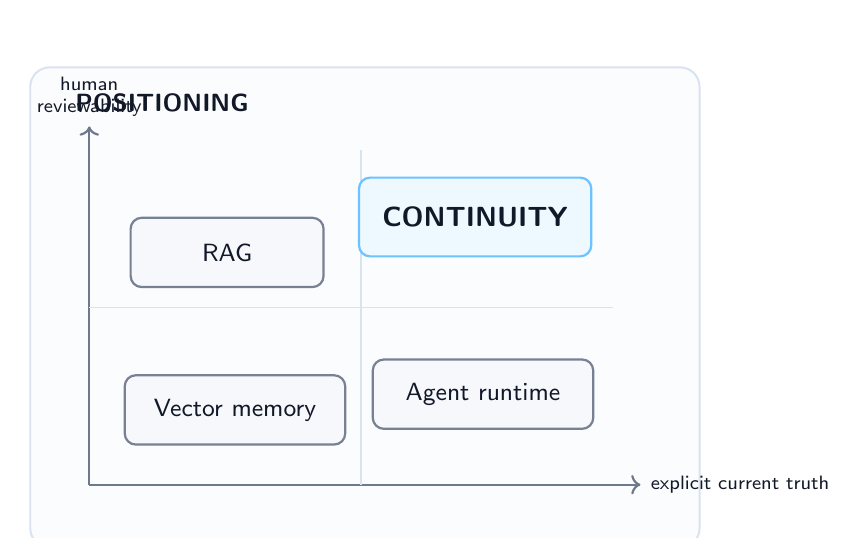
\begin{tikzpicture}[every node/.style={figlabel}]
\path[figpanel] (-0.75,-0.8) rectangle (7.75,5.3);
\node[figtitle, anchor=west] at (-0.3,4.85) {POSITIONING};
\draw[->, thick, BitSlate!85] (0,0) -- (7.0,0) node[right, figsmall] {explicit current truth};
\draw[->, thick, BitSlate!85] (0,0) -- (0,4.55) node[above,align=center, figsmall] {human\\reviewability};
\draw[BitLine] (0,2.25) -- (6.65,2.25);
\draw[BitLine] (3.45,0) -- (3.45,4.25);
\node[livebox, minimum width=2.95cm, minimum height=1.0cm, font=\sffamily\bfseries] at (4.9,3.4) {CONTINUITY};
\node[neutralbox, minimum width=2.45cm, minimum height=.88cm] at (1.75,2.95) {RAG};
\node[neutralbox, minimum width=2.8cm, minimum height=.88cm] at (1.85,0.95) {Vector memory};
\node[neutralbox, minimum width=2.8cm, minimum height=.88cm] at (5.0,1.15) {Agent runtime};
\end{tikzpicture}
\caption{CONTINUITY occupies a narrower niche than retrieval and orchestration layers.}
\label{fig:positioning-map}
\end{figure}


\subsection{Why Markdown remains the default}

Markdown is still the right starting substrate because it is inspectable, diffable, portable, and already understood by current coding agents. It also fails gracefully: when a file is wrong, a human can repair it with a text editor.

\subsection{Why Continuity is not just \RAG{} or a memory database}

\RAG{} retrieves possibly relevant material. CONTINUITY records mutable operational truth: what is currently true, what is next, and what evidence exists. Memory databases can complement that layer, but they do not remove the need for explicit state artifacts that humans can review.

\subsection{Why Continuity is not an agent runtime}

The repository cannot schedule workers, enforce permissions, or guarantee isolation by itself. Continuity is a control surface and a persistence convention. Runtime discipline still lives in the surrounding toolchain.

\subsection{Main limitation}

The design can collapse into paperwork. If the files become ceremonial, overlong, or stale, the system turns into a liability. That is why the paper repeatedly returns to one constraint: the defensible system is the smallest one that still preserves continuity.


\section{Conclusion}

Continuity argues for a small but durable shift in how coding agents work with repositories. The repository should not store code alone. It should also store the minimal state needed to let work survive a session boundary: current truth, active tasks, validated lessons, append-only history, and reviewable evidence.

That claim is strongest when it remains narrow. External memory research supports persistent state. Repository-local manifest practice shows that current tools already lean this way. Architecture and provenance research explain why the state should be inspectable. Security research explains why the same files cannot be trusted blindly. The resulting design stance is clear: keep the state layer compact, scoped, validated, and easy to delete. Anything more should earn its place by evidence.

\printbibliography
\appendix

\section{Appendix A: Minimal file templates}

\subsection*{Example \file{STATE.md}}
\begin{lstlisting}
# State

## System summary
Authentication service uses OAuth 2.1 with PKCE. Token refresh is server side.

## What changed recently
- Callback validation moved into auth middleware.
- Legacy refresh endpoint is deprecated but still present.

## Active constraints
- Do not change the token schema without migration notes.
- Any auth flow change requires integration tests.

## Next reconciliation point
Update after the current callback test suite finishes.
\end{lstlisting}

\subsection*{Example \file{TODO.md}}
\begin{lstlisting}
- [in-progress] Add callback replay protection
  owner: implementer-02
  evidence: artifacts/auth/replay-tests.txt

- [open] Remove legacy refresh endpoint after migration note lands
  dependency: callback replay protection
\end{lstlisting}


\section{Appendix B: Suggested lints}

\begin{itemize}
  \item Reject unresolved placeholders such as \file{\{\{VARIABLE\}\}} in trusted state files.
  \item Reject root manifests that exceed a configurable line or token budget.
  \item Warn when \file{STATE.md} contains stale timestamps or diary-style history.
  \item Warn when archives appear in default load lists.
  \item Reject nested files that weaken parent safety rules.
  \item Reject completed tasks that do not reference commits, tests, or artifacts.
  \item Warn when generated summaries are promoted without review metadata.
\end{itemize}

\end{document}